\chapter{含字母的计算与方程}\label{ch:g8:equations}

七年级已经引入了字母，并化简了简单的\omterm{def:g7:literal:def}{代数式}
（见\cref{ch:g7:literal}）。本章增加两项使代数变得强大的技能：
\emph{展开}括号的乘积，以及
\emph{解方程}，即求出隐藏在
字母背后的那个数。

\section{展开}

\begin{theorem}[单分配律与双分配律]\label{thm:g8:equations:expand}
对所有数，有：
\[
k(a + b) = ka + kb,
\qquad
(a + b)(c + d) = ac + ad + bc + bd .
\]
\end{theorem}

\begin{proof}
第一条法则即\cref{thm:g7:priorities:distributivity}，
其中符号也要考虑：$k$ 与各项可能为负（见
\cref{ch:g8:negprod}）。对于第二条，两次应用第一条法则，
并把 $(c + d)$ 看作一个数：
\[
(a + b)(c + d) = a(c + d) + b(c + d) = ac + ad + bc + bd .
\qedhere
\]
\end{proof}

\begin{example}\label{ex:g8:equations:expand}
注意每一项的符号：
\begin{align*}
3(2x - 5) &= 6x - 15, \\
-2(4x - 7) &= -8x + 14
&& \text{（前面的负号使两项的符号都改变）}, \\
(x + 3)(x + 5) &= x^2 + 5x + 3x + 15 = x^2 + 8x + 15, \\
(2x - 1)(x - 4) &= 2x^2 - 8x - x + 4 = 2x^2 - 9x + 4 .
\end{align*}
\end{example}

\begin{omfigure}
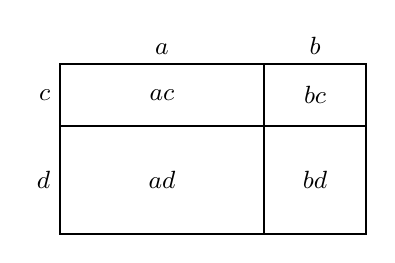
\begin{tikzpicture}[scale=0.72]
  \draw[thick] (0,0) rectangle (5.4,3.0);
  \draw[thick] (3.6,0) -- (3.6,3.0);
  \draw[thick] (0,1.9) -- (5.4,1.9);
  \node[font=\small] at (1.8,2.45) {$ac$};
  \node[font=\small] at (4.5,2.45) {$bc$};
  \node[font=\small] at (1.8,0.95) {$ad$};
  \node[font=\small] at (4.5,0.95) {$bd$};
  \node[above, font=\small] at (1.8,3.0) {$a$};
  \node[above, font=\small] at (4.5,3.0) {$b$};
  \node[left, font=\small] at (0,2.45) {$c$};
  \node[left, font=\small] at (0,0.95) {$d$};
\end{tikzpicture}

{\small 从\omterm{def:g6:measure:area}{面积}看双重分配律：长方形
$(a+b) \times (c+d)$ 被分成四个较小的长方形，
每个小长方形对应展开式中的一项。}
\end{omfigure}

\begin{method}[展开并化简]\label{met:g8:equations:reduce}
\begin{enumerate}
  \item 展开每一个乘积，并写出每一项的符号；
  \item 合并同类项（$x^2$ 与 $x^2$，$x$ 与 $x$，
        数与数）；
  \item 用数值检验：例如在原式与化简结果中代入 $x = 2$，
        若两者结果相等，大多数错误便能被发现。
\end{enumerate}
\end{method}

\section{解方程}

\begin{definition}[方程]\label{def:g8:equations:def}
含未知数的等式称为\emph{方程}\index{方程}，
未知数记为 $x$（或任意字母）。\emph{求解}方程是指求出
使等式成立的所有 $x$ 的值，
这些值即方程的\emph{解}。
\end{definition}

\begin{theorem}[等式的平衡法则]\label{thm:g8:equations:balance}
方程在下列情形下，解完全不变：
\begin{enumerate}
  \item 等式两边同时加上（或减去）同一个数；
  \item 等式两边同时乘以（或除以）同一个
        \emph{非零}的数。
\end{enumerate}
\end{theorem}
\admitted

\begin{omfigure}
\begin{tikzpicture}[scale=0.9]
  \draw[thick] (0,0) -- (0,0.5);
  \draw[thick] (-2.6,0.5) -- (2.6,0.5);
  \draw[thick] (-0.5,0) -- (0.5,0);
  \draw[thick] (-2.2,0.5) -- (-2.2,0.75);
  \draw[thick] (2.2,0.5) -- (2.2,0.75);
  \draw[omDef, fill=omDef!15] (-2.8,0.75) rectangle (-1.6,1.45);
  \node[font=\small] at (-2.2,1.1) {$x{+}3$};
  \draw[omThm, fill=omThm!15] (1.75,0.75) rectangle (2.65,1.45);
  \node[font=\small] at (2.2,1.1) {$8$};
  \node[below, font=\small] at (0,-0.25)
    {从两盘各拿走 $3$：$x = 5$};
\end{tikzpicture}

{\small 方程好比一架天平：对其中一盘所做的操作，
必须同样对另一盘进行，天平的平衡——即等式——
依然保持。}
\end{omfigure}

\begin{method}[解一元一次方程]\label{met:g8:equations:solve}
\begin{enumerate}
  \item 必要时，展开每一边并合并同类项；
  \item 两边同时加上或减去同一个数，使含 $x$ 的项集中到一边，
        常数项集中到另一边；
  \item 合并同类项，再在两边同时除以 $x$ 的系数；
  \item \emph{检验}：把求得的值代入原来的
        方程，看等式是否成立。
\end{enumerate}
\end{method}

\begin{example}\label{ex:g8:equations:solve}
解方程 $7x - 5 = 4x + 16$：
\begin{align*}
7x - 5 &= 4x + 16 \\
7x - 4x &= 16 + 5
&& \text{（两边同时加 $5$，减 $4x$）} \\
3x &= 21 \\
x &= 7 && \text{（两边同时除以 3）。}
\end{align*}
验算：左边 $7 \times 7 - 5 = 44$；右边
$4 \times 7 + 16 = 44$。方程的解是 $7$。
\end{example}

\begin{example}[含括号与负数的情形]\label{ex:g8:equations:brackets}
解方程 $3(x - 4) = 5 - 2(x + 1)$：
\begin{align*}
3x - 12 &= 5 - 2x - 2 && \text{（两边同时展开）} \\
3x - 12 &= 3 - 2x && \text{（合并同类项）} \\
5x &= 15 && \text{（两边同时加上 $2x + 12$）} \\
x &= 3 .
\end{align*}
验算：$3(3 - 4) = -3$ 且 $5 - 2(3+1) = 5 - 8 = -3$。\quad 解：
$3$。
\end{example}

\begin{method}[用方程解应用题]\label{met:g8:equations:problem}
\begin{enumerate}
  \item 选择未知数：“设 $x$ 为\dots”（所求的量，
        或与之相关的较简单的量）；
  \item 将题目中的叙述译为方程；
  \item 解方程；
  \item 解释结果：用一句话回答原问题，写明
        单位，并对照题意检验答案。
\end{enumerate}
\end{method}

\begin{example}\label{ex:g8:equations:problem}
卢卡斯比他的姐姐大 $4$ 岁；两人的年龄之和为
$26$。设 $x$ 为姐姐的年龄，则卢卡斯的年龄为 $x + 4$，于是
\[
x + (x + 4) = 26
\ \Longrightarrow\
2x + 4 = 26
\ \Longrightarrow\
2x = 22
\ \Longrightarrow\
x = 11 .
\]
姐姐为 $11$ 岁，卢卡斯为 $15$ 岁。验算：$11 + 15 = 26$，且
$15 - 11 = 4$。
\end{example}

\section{大小关系与不等式}

\begin{proposition}[运算与大小关系]\label{prop:g8:equations:order}
不等式两边同时加上同一个数，不等号方向保持不变；
两边同时乘以一个\emph{正数}，不等号方向保持不变；
乘以一个\emph{负数}时，不等号方向\emph{改变}：
\[
2 < 5 \ \text{ 但是 }\ (-1) \times 2 > (-1) \times 5 .
\]
\end{proposition}
\admitted

\begin{example}\label{ex:g8:equations:inequality}
解不等式 $5 - 2x \leq 11$：两边同时减去 $5$，得 $-2x \leq 6$；
两边同时除以 $-2$，并\emph{改变不等号方向}：$x \geq -3$。所有
大于或等于 $-3$ 的数都是解——方程通常只有一个解，
而不等式的解是一整条半直线。
\end{example}

\section{练习}

\begin{exercise}[$\star$]\label{exo:g8:equations:1}
展开并合并同类项：
\[
5(2x + 3), \qquad
-3(4x - 1), \qquad
2(3x - 2) + 4(x + 5).
\]
\end{exercise}

\begin{exercise}[$\star$]\label{exo:g8:equations:2}
展开并合并同类项：
\[
(x + 2)(x + 7), \qquad
(3x + 1)(2x - 5), \qquad
(x - 4)(x - 6).
\]
\end{exercise}

\begin{exercise}[$\star$]\label{exo:g8:equations:3}
判断 $x = 3$ 是否为方程 $4x - 5 = 7$、$2x + 1 = x + 4$ 的解，
以及是否为方程 $x^2 = 6x - 9$ 的解？（代入并比较等式两边。）
\end{exercise}

\begin{exercise}[$\star$]\label{exo:g8:equations:4}
解下列方程，并进行检验：
\[
x + 9 = 4, \qquad
5x = -35, \qquad
\frac{x}{3} = 8, \qquad
2x - 7 = 13 .
\]
\end{exercise}

\begin{exercise}[$\star$]\label{exo:g8:equations:5}
解下列方程：
\[
6x + 5 = 2x + 25, \qquad
9 - 4x = x - 11, \qquad
3(x + 2) = 2x + 11 .
\]
\end{exercise}

\begin{exercise}[$\star$]\label{exo:g8:equations:6}
解方程 $4(2x - 3) = 5(x + 6)$，先展开再求解，
并检验你的解。
\end{exercise}

\begin{exercise}[$\star$]\label{exo:g8:equations:7}
列出方程并求解：“一个数的三倍减去 $8$ 等于
$19$”；“一个数的两倍增加 $5$ 后，等于这个数增加
$12$”。
\end{exercise}

\begin{exercise}[$\star\star$]\label{exo:g8:equations:8}
一个长方形的长比宽多 $5$ cm，其\omterm{def:g6:measure:perimeter}{周长}为
$58$ cm。设 $x$ 为宽，列出方程并求解，
并求出长和宽。
\end{exercise}

\begin{exercise}[$\star\star$]\label{exo:g8:equations:9}
三个连续整数的和为 $141$。记中间的数为
$n$，求出这三个数。
\end{exercise}

\begin{exercise}[$\star\star$]\label{exo:g8:equations:10}
解下列不等式，并描述其解集：
\[
3x + 4 > 19, \qquad
7 - 2x \geq 1, \qquad
5(x - 1) < 2x + 7 .
\]
\end{exercise}

\begin{exercise}[$\star\star$]\label{exo:g8:equations:11}
米娅有存款 $140$ 欧元，每月增加 $15$ 欧元；汤姆
有 $200$ 欧元，每月增加 $10$ 欧元。经过几个月后，
米娅的存款严格多于汤姆的存款？（列出不等式。）
\end{exercise}

\begin{exercise}[$\star\star\star$]\label{exo:g8:equations:12}
解方程 $\dfrac{x + 3}{4} = \dfrac{2x - 1}{5}$。
（两边同乘公\omterm{def:g4:fractions:def}{分母} $20$，再按常规方法求解；
并把解代入原方程检验。）
\end{exercise}

\section{问题：乘法公式与
奇数的阶梯}

\begin{problem}[{周末问题——$(a+b)^2$，$(a-b)^2$，
$(a+b)(a-b)$，以及奇数求和 $1 + 3 + 5 + \dots + (2n-1) = n^2$}]
\label{pb:g8:equations:1}
三个展开式十分常用，代数中人们把它们
熟记于心，它们被称为\emph{乘法公式}。本题
由双重分配律推出它们，
（见\cref{thm:g8:equations:expand}），将它们变成心算的
超能力，用它们证明一个关于\omterm{def:g3:numbers:evenodd}{奇数}的漂亮事实，
最后求解一类全新的方程：
含平方项的方程。

\medskip
\noindent\textbf{第一部分——三个乘法公式。}
\begin{enumerate}
  \item 展开 $(a + b)^2 = (a + b)(a + b)$ 并化简，证明
        \[
        (a + b)^2 = a^2 + 2ab + b^2 .
        \]
  \item 类似地证明另外两个公式：
        \[
        (a - b)^2 = a^2 - 2ab + b^2,
        \qquad
        (a + b)(a - b) = a^2 - b^2 .
        \]
  \item 画一个边长为 $a + b$ 的正方形，将每条边分为 $a$
        和 $b$ 两段，并将正方形切成四块。
        图中各部分分别对应
        第一个公式中的哪一项？
  \item 心算：利用这些公式计算，
        不列出任何乘法算式，求下列各式的值：
        \[
        101^2, \qquad 99^2, \qquad 49 \times 51 .
        \]
  \item 一个经典陷阱：佐伊写出“$(a + b)^2 = a^2 + b^2$”。
        取 $a = 3$，$b = 4$ 检验她的公式，并在
        第 3 小题的图上说明，她的公式
        遗漏了哪些部分。
\end{enumerate}

\medskip
\noindent\textbf{第二部分——\omterm{def:g3:numbers:evenodd}{奇数}的阶梯。}
\begin{enumerate}[resume]
  \item 依次计算 $1$、$1 + 3$、$1 + 3 + 5$，接着
        $1 + 3 + 5 + 7$，再算 $1 + 3 + 5 + 7 + 9$。你发现
        这些结果有什么规律？
  \item 说明为什么第 $n$ 个\omterm{def:g3:numbers:evenodd}{奇数}是 $2n - 1$（检验：
        $n = 1, 2, 3$ 分别给出 $1, 3, 5$）。
  \item 利用第一部分中的一个公式展开并化简
        $(n + 1)^2 - n^2$。这个结果与
        第 7 小题有什么关系？
  \item 第 8 小题指出：要从边长为 $n$ 的正方形
        变为边长为 $n + 1$ 的正方形，恰好需要添加下一个\omterm{def:g3:numbers:evenodd}{奇数}
        个单位方格，即沿两条边加一个 L 形的框，
        再加上拐角处的方格。从 $1 = 1^2$ 出发，逐层
        扩大正方形，解释为什么
        \[
        1 + 3 + 5 + \dots + (2n - 1) = n^2 :
        \]
        即前 $n$ 个\omterm{def:g3:numbers:evenodd}{奇数}之和是第 $n$ 个平方数。
  \item 不必逐个相加，推出：
        $1 + 3 + 5 + \dots + 99$ 的值；以及从 $1$ 开始，
        需要取多少个\omterm{def:g3:numbers:evenodd}{奇数}相加，和恰好为 $400$？
\end{enumerate}

\medskip
\noindent\textbf{第三部分——含平方的方程。}
\begin{enumerate}[resume]
  \item 识别 $x^2 + 6x + 9$ 中的一个乘法公式，并
        解方程 $x^2 + 6x + 9 = 0$。
  \item 借助 \cref{thm:g8:negprod:rules}
        中的符号与绝对值规则，说明为什么两个数之积
        \emph{只有当}其中一个因式为零时，积才可能为零。
        利用这一结论解方程 $(x - 2)(x + 5) = 0$。
  \item 解方程 $x^2 = 49$：把所有项移到一边，
        再用第三个公式分解 $x^2 - 49$。这个方程有几个解？
        它与本章到目前为止所解的每个方程有何
        不同？
  \item 在\cref{exo:g8:equations:3}中你验证过 $x = 3$ 是
        方程 $x^2 = 6x - 9$ 的解。现证明它是
        \emph{唯一}的解：把各项移到一边，识别
        一个乘法公式，并作出结论。
  \item 压轴：心算 $2026^2 - 2025^2$，并
        利用乘法公式说明为什么两个相邻平方数之差
        总是这两个数的和
——正是第 8 小题的内容。
\end{enumerate}
\end{problem}
